\section{Deconstruction}
\label{sec:deconstruction}

\subsection{What must be explained}

Section~\ref{sec:apparent} leaves three facts to explain: a strong negative
$\beta_h(0.01)$ that deepens from \BetaQoneHzero{} to \BetaQoneHtwelve{}
over twelve hours; a tail-to-median ratio of \RatioTailMedImpact{} on
impact; and a left tail that appears to respond more than the right. Three
readings compete. The first is genuine downside-specific amplification, the
leverage-cycle interpretation; the second is a genuine but \emph{symmetric}
volatility channel, misread; the third is a mechanical artifact of the overlapping
cumulative design. We do not adjudicate by assertion. Each alternative is
confronted with a test built to manufacture the stylized fact under
a known null: if the test reproduces the fact, the fact is not a signature
of the first reading. Two distinctions organize the section. The \emph{level} of $\beta$
and the \emph{shape} of the response are separate questions. Level
means the magnitude of $|\beta_h(0.01)|$ (the scale channel of
Section~\ref{sec:method-controls}, tested by the permutation nulls); shape
means the left-minus-right gap $g_h = |\beta_h(0.01)| -
|\beta_h(0.99)|$\footnote{The gap pairs each tail quantile with its
equidistant mirror: $0.01$ with $0.99$, and the headline ratio of
Section~\ref{sec:apparent} pairs $0.01$ with $0.95$. The reporting grid
stops at $0.95$, but $0.99$ is estimated as part of the tail-inference set
(Section~\ref{sec:method-inference}); the headline ratio uses $0.95$ as the
rhetorical object, while the rigorous left-versus-right test below uses the
true mirror $0.99$.} (tested by the placebo). A coefficient can
therefore be genuine in level yet symmetric in shape, and that, we will conclude, is
exactly what the data say. And ETH-specificity is a separate question again, tested by
replacing the outcome altogether.

\subsection{The symmetric placebo}
\label{sec:placebo}

We simulate a world that is symmetric by construction and re-run the exact
estimation kernel on it. Returns are rebuilt as $r^{\text{sim}}_t = m_t \pm
|\hat{\varepsilon}_t|$, where $m_t$ is the fitted conditional mean and the
sign is an independent Rademacher draw, the sign-flip construction of
the wild-bootstrap literature \citep{wu1986,liu1988,davidson2008}. The
simulated world thus has \emph{zero skew by construction} at every point in
time, while preserving the empirical magnitude sequence exactly: the full
fat-tailed, volatility-clustered path of $|\hat{\varepsilon}_t|$, with no
volatility model imposed at all. Because the sign-flip removes asymmetry
while leaving the volatility path untouched, any left--right gap this world
produces is, by construction, what symmetric heteroskedasticity alone
manufactures through extreme quantiles. A gap that the real data
merely matches therefore cannot be evidence of real downside skew. Only the
dependent variable is simulated;
the shock and all controls are the real series. Each of 500 simulated
panels is passed through the identical quantile-LP kernel, and the
statistic of interest is the left--right gap $g_h = |\beta_h(0.01)| -
|\beta_h(0.99)|$. The level of $|\beta|$ is expected to survive (the
volatility path is real, which is the point), so the test bites on the
\emph{asymmetry}, which the design rules out as a property of the data.

The zero-skew world reproduces the observed asymmetry everywhere
(Figure~\ref{fig:placebo}). At twelve hours the real gap
($\GapRealHtwelve$) sits near the center of the placebo distribution
($[\GapBandLoHtwelve, \GapBandHiHtwelve]$); on impact the real gap
($\GapRealHzero$) lies within the symmetric band
($[\GapBandLoHzero, \GapBandHiHzero]$). There is no real impact gap either. Nor is this
verdict an artifact of the band's width. Sweep the placebo's tail
thickness across a variance-preserving family, from thin- to
heavy-tailed, and the real gap stays inside the symmetric band at the data's
own tail thickness and under every heavier tail; it escapes only when the
simulated world is forced thinner-tailed than the data, an artificially
narrow band that under-represents the spread the returns actually carry. A
dose-response sweep of the heteroskedasticity \emph{amplitude} (tracing
the manufactured gap against a tail-thickness parameter) would only
confirm the monotonicity of a mechanism the placebo already exhibits at the
data's own heteroskedasticity, at the cost of an arbitrary parametric family,
and is omitted. A vol-model-scaled variant, in which standardized magnitudes are permuted
across dates and rescaled by a fitted volatility path (a shock-driven
rolling specification and a shock-agnostic GARCH(1,1), two
distinct designs), delivers the same verdict in all fourteen
model-horizon cells. The observed left--right asymmetry is therefore what
symmetric heteroskedasticity looks like through extreme quantiles of
cumulative returns, the mechanism demonstrated for macroeconomic tail risk by \citet{carriero2024}, instantiated here on asset returns. Consistently,
\citet{brownlees2021} find that a symmetric GARCH rivals
quantile-regression tail-risk models out of sample: the scale channel does
the work. One reading discipline applies. Where the placebo occasionally
generates more asymmetry than observed, the correct statement is
that the real gap does not exceed what a zero-skew world generates; the
test is one of non-exceedance, not of equality.

\begin{figure}[t]
\centering
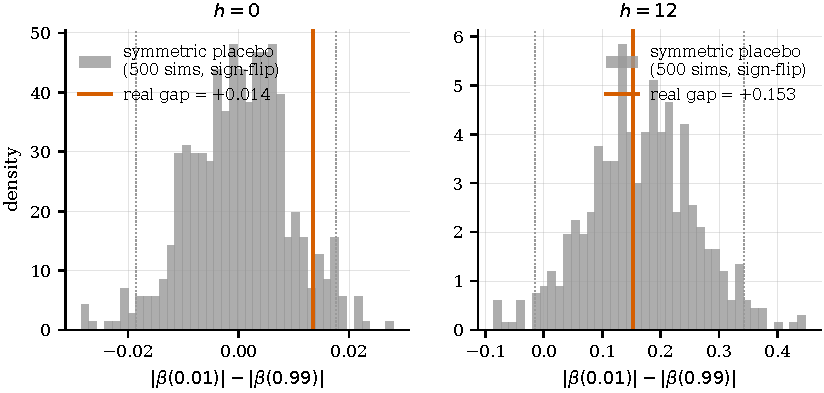
\includegraphics[width=\textwidth]{../paper/figures/fig4_placebo_gap_distribution}
\caption{Distribution of the left--right tail gap $|\beta(0.01)| - |\beta(0.99)|$ across 500 zero-skew sign-flip placebo worlds (grey; dotted lines mark the 2.5th/97.5th percentiles), against the real gap (vertical line), on impact and at twelve hours. The real asymmetry is indistinguishable from what a symmetric world produces.}
\label{fig:placebo}
\end{figure}

\subsection{The permutation nulls}
\label{sec:purenull}

The placebo addresses shape. The level question, whether the deepening
$\beta_h(0.01)$ is a mechanical artifact of the overlapping cumulative design
\citep{hodrick1992,boudoukh2008,valkanov2003}, is answered with two
permutation nulls run at 500 draws each, and reported jointly as a
guard against null-shopping. The conservative null circularly shifts the
shock series, preserving its marginal distribution and autocorrelation
(and the real, heteroskedastic dependent variable) while severing only its
alignment with returns. The coarser null reshuffles the return innovations
themselves, destroying their serial dependence; the two designs bracket
what a ``no information'' world can mean here, and diagnostics of what
each null preserves and destroys are recorded with the artifacts.

Both nulls return the same verdict (Figure~\ref{fig:purenull}). Mechanical
noise accounts for a minority of the observed coefficient at every
horizon: the null-to-real magnitude ratio at twelve hours is
\PnCircHtwelve{} under the conservative null and \PnInnovHtwelve{} under
the coarser one, rising to at most \PnCircHtwentyfour{} at twenty-four
hours. The signed mean of the null distribution is essentially zero
throughout (e.g.\ \PnCircSignedHtwelve{} at twelve hours, against a real
coefficient of \BetaQoneHtwelve): the overlap inflates the
\emph{dispersion} of tail estimates, it does not push them downward.
And the real coefficient lies outside the null band
($[\PnCircQloHtwelve, \PnCircQhiHtwelve]$ at twelve hours) at every
horizon, with permutation $p$-values below $0.005$ through eighteen hours
and \PnCircPermPHtwentyfour{} at twenty-four. The level is
overwhelmingly real.\footnote{The medium-horizon \emph{magnitude} is
separately sensitive to the MakerDAO coverage gap (Appendix~\ref{app:data});
the permutation nulls certify only that the deepening is not a mechanical
artifact of overlap, a distinct question from coverage.} This matters in both
directions. It removes the
artifact reading as a primary explanation, and it sharpens the burden
on interpretation: the coefficient is real, so the question is entirely
what it means.

\begin{figure}[t]
\centering
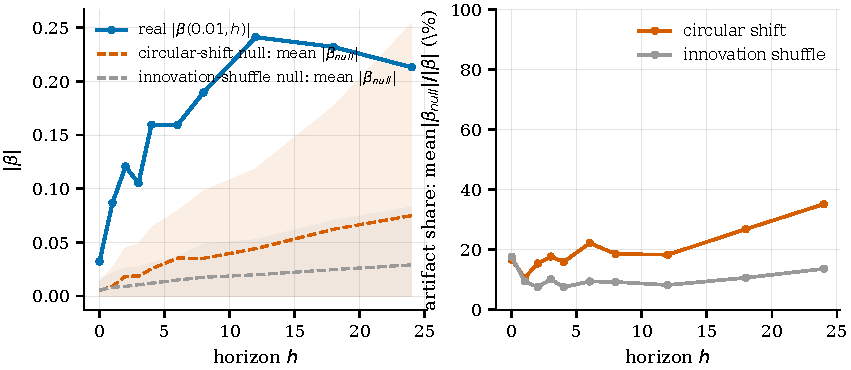
\includegraphics[width=\textwidth]{../paper/figures/fig9_pure_null_dual}
\caption{Dual permutation nulls. Left: the real $|\beta_h(0.01)|$ against
the mean null magnitude under each construction (shaded: null bands).
Right: the null-to-real ratio by horizon, a minority share everywhere,
under both nulls.}
\label{fig:purenull}
\end{figure}

\subsection{The overlap artifact}
\label{sec:overlap}

If the overlapping cumulative construction misleads about \emph{shape}
rather than level, the cleanest demonstration is to remove it. The
exceedance regressions of Section~\ref{sec:survives} use per-period (non-overlapping)
tail-violation indicators; their paired asymmetry $\Delta_h =
\beta^{\text{down}}_h - \beta^{\text{up}}_h$ is null at every horizon
(at twelve hours, $p = \DeltaExcHtwelveP$). Re-running the same
construction on overlapping cumulative returns manufactures a significant
asymmetry at exactly the horizons where the naive reading is most
dramatic ($\Delta_{12} = \DeltaExcCumHtwelve$, $p = \DeltaExcCumHtwelveP$;
Figure~\ref{fig:exceedance}, right panel). Same data, same controls, same
estimator family. The only difference is the overlap. The
horizon-dependent skewness that cumulation fabricates
\citep{neuberger2021,farago2023} is not a theoretical curiosity here; it is
visible in one comparison.

One might worry the null is an artifact of conditioning, that holding the
controls fixed is what suppresses the asymmetry. Re-estimating the effect on
the \emph{marginal} return quantile, by the unconditional-quantile (RIF)
method, answers it. On the density-normalized scale the combined
tail-widening at impact is large (\RifVolWideningImpact), both tails opening
together, the volatility channel again, while the down-versus-up asymmetry
recovered from the same estimates reproduces the conditional exceedance
($\Delta_0 = \DeltaExcImpact$) to machine precision at every horizon. The
agreement is partly algebraic: RIF-OLS with these
controls is the conditional linear-probability model up to the density
factor, so it confirms the null rather than re-deriving it independently.
What the unconditional lens adds is the one distinct object,
the large symmetric widening, and it points the same way.

\subsection{The headline ratio}

The ``\RatioTailMedImpact$\times$'' headline deserves a closer look,
because it is rhetorically the strongest number in
Section~\ref{sec:apparent} and statistically the emptiest. Volatility
widens both tails but does not move the center: $\beta_h(0.50) \approx 0$
is what a scale channel implies (and what the silent OLS mean
regression already said). A tail-to-median ratio with a near-zero
denominator explodes mechanically; it measures ``the median is immobile,''
not ``the downside is special.'' Diverging quantile slopes, the fanning
of Figure~\ref{fig:irf}, are the textbook signature of
heteroskedasticity, not of shape change \citep{koenker1982,machado2000}.
And the correct contrast, left tail against right tail, is the one
the ratio hides: $\beta_{12}(0.05) = \BetaFiveHtwelve$ against
$\beta_{12}(0.95) = \BetaNinetyFiveHtwelve$, both tails moving. At
horizons beyond impact the median itself drifts positive
($\beta_{12}(0.50) = \BetaMedHtwelve$), and the ratio collapses to
\RatioTailMedHtwelve$\times$. The headline number is also
impact-specific.

\subsection{The BTC-outcome placebo}
\label{sec:btc}

A final alternative survives the tests above: perhaps the response is
real and symmetric, and still specifically about ETH's DeFi collateral
channel. The sharpest test replaces the outcome. We re-run the full
quantile local projection, identical shock and horizons, with
Bitcoin returns as the dependent variable (the cross-asset control
becoming ETH's return, by symmetry; BTC has no comparable ETH-collateral
DeFi channel). The ETH signature replicates on Bitcoin in every respect
(Figure~\ref{fig:btc}): $\beta^{\text{BTC}}_0(0.01) = \BtcBetaQoneHzero$
on impact, deepening to $\BtcBetaQoneHtwelve$ at twelve hours, a
near-parallel profile at \BtcOverEthHzero{} of the ETH magnitude on impact
and \BtcOverEthHtwelve{} at twelve hours, with an even more extreme
tail-to-median ratio on impact (\BtcRatioTailMedImpact$\times$, BTC's
median response being essentially zero). The naive signature is therefore
not evidence of an ETH-specific DeFi channel. It is what generic crypto
stress looks like through this lens, on any correlated asset. The residual
claim of ETH specificity is accordingly demoted: BTC carries most of the
signature, and no ETH-specific increment large enough to drive the result
survives. The methodological lesson gains generality, since the
misreading would afflict any asset regressed on any stress-correlated
flow.

\begin{figure}[t]
\centering
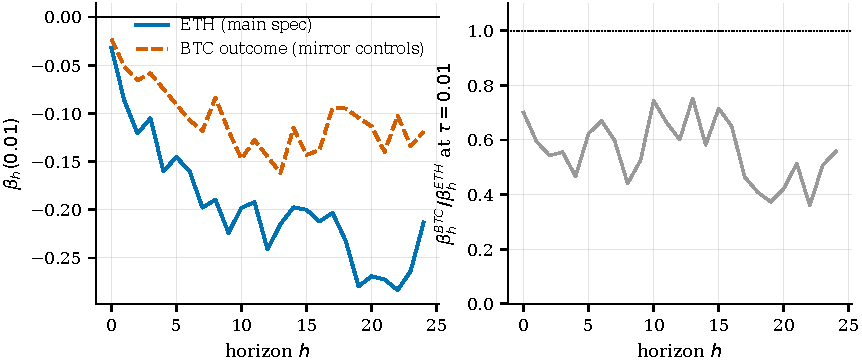
\includegraphics[width=\textwidth]{../paper/figures/fig8_btc_vs_eth}
\caption{BTC-outcome placebo. Left: $\beta_h(0.01)$ profiles, ETH (main specification) and BTC as outcome (mirror controls). Right: the BTC-to-ETH coefficient ratio by horizon. The apparent ``downside-amplification'' signature replicates on an asset without the ETH-collateral channel.}
\label{fig:btc}
\end{figure}

\subsection{The portable detection battery}
\label{sec:lesson}

What is new here, and what is borrowed, should be stated carefully. The
mechanism, symmetric and time-varying volatility producing apparent
downside sensitivity in quantile models, is established in the
macroeconomic Growth-at-Risk setting by \citet{carriero2024}; the overlap
pathologies of long-horizon regressions are classic
\citep{hodrick1992,boudoukh2008,valkanov2003}; scale-versus-shape in
quantile regression goes back to \citet{koenker1982} and
\citet{machado2000}. What is new, to our knowledge, is the
\emph{conjunction} in which all four ingredients meet (asset returns,
overlapping cumulation, quantile local projections, and the extreme tail)
together with a diagnostic battery that detects the trap on real data:
a model-free zero-skew placebo for shape, dual permutation nulls for
level, a per-period-versus-cumulative comparison that exhibits the
artifact directly, a cross-asset outcome placebo for specificity, and a
planted-cascade positive control under which the equivalence apparatus
recovers a downside asymmetry at twice the actionable threshold and stays
silent below it, so the bounded null it returns is power-confirmed, not
power-absent. The lesson travels: any literature that regresses extreme quantiles of
cumulative returns on stress-correlated regressors, and the nascent
empirical DeFi literature is about to be one, can produce
``endogenous fragility'' of this apparent strength from a symmetric
volatility channel.

\subsection{Reconciliation}

The reconciled reading of Section~\ref{sec:apparent} is now complete. In
\emph{level}, $\beta_h(0.01)$ is overwhelmingly genuine: both
permutation nulls leave mechanical noise a minority share, with no signed
bias. In \emph{shape}, the asymmetry is not real. A zero-skew world
reproduces the entire left--right gap at every horizon, the per-period
construction shows both tails loading equally, and the headline ratio is
an artifact of an immobile median. In \emph{specificity}, the signature
replicates on Bitcoin. What the naive analysis detected is a real,
symmetric, generic-crypto volatility response, the second moment
dressed up as downside fragility. What remains to establish is what
survives on the positive side, and how tightly the null can be bounded;
that is Section~\ref{sec:survives}.